%%%%%%%%%%%%
%% Please rename this main.tex file and the output PDF to
%% [lastname_firstname_graduationyear]
%% before submission.
%%%%%%%%%%%%

\documentclass[12pt]{caltech_thesis}
\usepackage[hyphens]{url}
\usepackage{lipsum}
\usepackage{graphicx}
\usepackage{xcolor}

%\usepackage{todonotes}

%% Tentative: newtx for better-looking Times
\usepackage[utf8]{inputenc}
\usepackage[T1]{fontenc}
\usepackage{newtxtext,newtxmath}

% Must use biblatex to produce the Published Contents and Contributions, per-chapter bibliography (if desired), etc.
\usepackage[
    backend=biber,natbib,
    %backend=natbib,
    % IMPORTANT: load a style suitable for your discipline
    style=authoryear-comp,
    doi=False,
    bibstyle=apj
]{biblatex}
\renewcommand*{\nameyeardelim}{\addspace}
%\usepackage{natbib}
%\bibliographystyle{apj}
\newcommand{\todo}[3]{{\color{#2} \emph{#1} TO DO: #3}}
\newcommand{\btmtodo}[1]{\todo{BEN}{red}{#1}}

\renewcommand{\d}[1]{\ensuremath{\operatorname{d}\!{#1}}}
\newcommand{\rsun}{{R$_\odot$}}
\newcommand{\msun}{{M$_\odot$}}
\newcommand{\rstar}{{R$_*$}}
\newcommand{\mstar}{{M$_*$}}
\newcommand{\kep}{{\textit Kepler}}
\newcommand{\KT}{{\textit K2}}

\newcommand{\aj}{AJ}
\newcommand{\pasp}{PASP}
\newcommand{\apj}{ApJ}
\newcommand{\aap}{A\%A}
\newcommand{\mnras}{MNRAS}
\newcommand{\sci}{Science}
\newcommand{\nat}{Nature}


% Name of your .bib file(s)
\addbibresource{exopapers.bib}
\addbibresource{example.bib}

\begin{document}

% Do remember to remove the square bracket!
\title{Low-Mass Stars and Their Companions}
\author{Benjamin Tyler Montet}

\degreeaward{Doctor of Philosophy}                 % Degree to be awarded
\university{California Institute of Technology}    % Institution name
\address{Pasadena, California}                     % Institution address
\unilogo{caltechseal2.png}                                 % Institution logo
\copyyear{2017}  % Year (of graduation) on diploma
\defenddate{July 18, 2016}          % Date of defense

\orcid{0000-0001-7516-8308}

%% IMPORTANT: Select ONE of the rights statement below.
%\rightsstatement{All rights reserved\todo[size=\footnotesize]{Choose one from the choices in the source code!! And delete this \texttt{todo} when you're done that. :-)}}
 \rightsstatement{All rights reserved except where otherwise noted}
% \rightsstatement{Some rights reserved. This thesis is distributed under a [name license, e.g., ``Creative Commons Attribution-NonCommercial-ShareAlike License'']}

%%  If you'd like to remove the Caltech logo from your title page, simply remove the "[logo]" text from the maketitle command
\maketitle[logo]
%\maketitle

\begin{acknowledgements} 	 
   People to thank: John + group. Brendan Bowler, Justin, Luan, 
   Hogg, DFM, Ruth. 
   Ian, Dawn, Ryan, Jieun, Aaron and Jason
   Cahill department and traditions - see Sirio's.
   Antonija + Mislav, Trevor, Allison, Yi. Matt, Sirio, Gwen and Drew, Ryan.
   Committee, Patrick and Anu
   Laura
   Parents
   
\end{acknowledgements}

\begin{abstract}
   [This abstract must provide a succinct and informative condensation of your work. Candidates are welcome to prepare a lengthier abstract for inclusion in the dissertation, and provide a shorter one in the CaltechTHESIS record.]
\end{abstract}

%% Uncomment the `iknowhattodo' option to dismiss the instruction in the PDF.
%\begin{publishedcontent}%[iknowwhattodo]
% List your publications and contributions here.
%\nocite{Cahn:etal:2015}
%\end{publishedcontent}

\tableofcontents
\listoffigures
\listoftables
%\printnomenclature

\mainmatter

\chapter{Introduction}

\section{M Dwarfs: The Silent Majority}
For much of the timescale of stellar astrophysics research, to a fanatic 
of M dwarf stars their history is a story of neglect and underappreciation.
The first spectrum of an M dwarf was obtained only 100 years ago when 
\citet{Adams13} collected an observation of the M+M binary Groombridge 34.
The oldest known surviving diagram plotting stellar absolute magnitude against spectral type \citep{Russell14}, now known as a Hertsprung-Russell Diagram, includes hundreds of stars, as shown in Figure \ref{fig:HR}.
Today we know that M dwarfs make up approximately 75\% of the stars in the galaxy,
yet only $\sim$5\% of the stars included in Russell's figure are listed as
spectral type M.



\begin{figure}[hbt!]
\centering
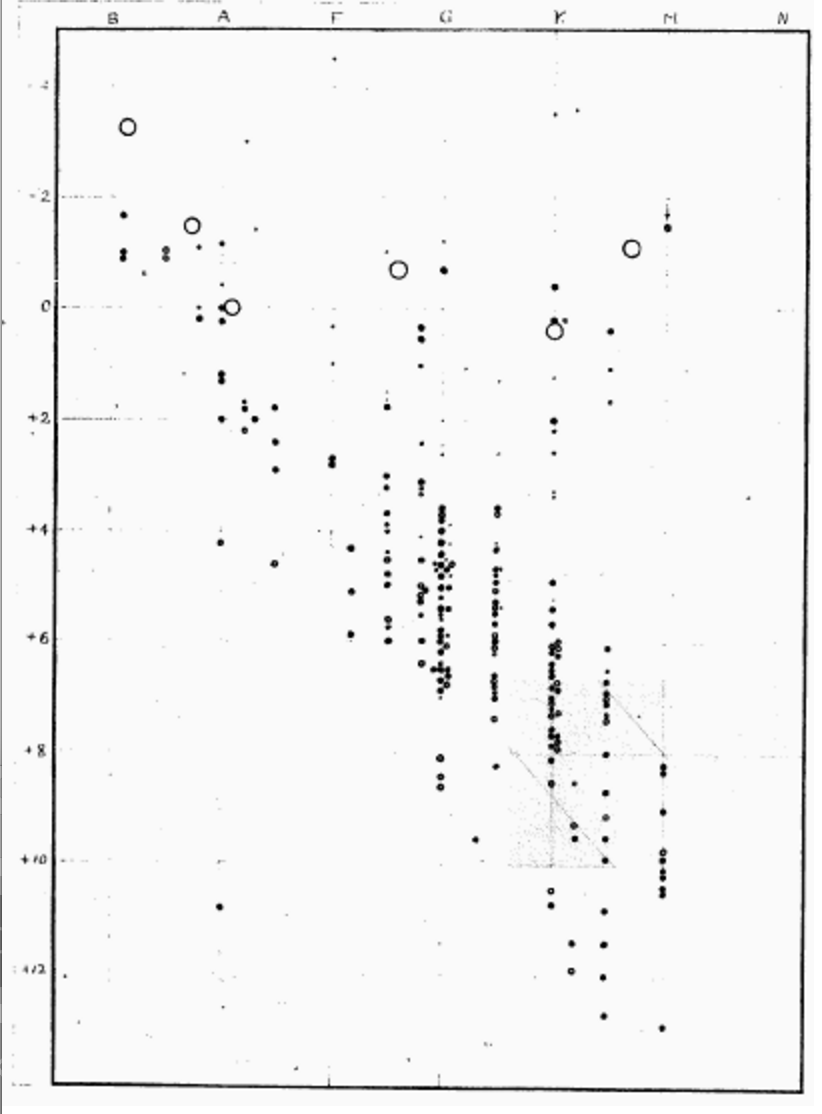
\includegraphics[width=.5\textwidth]{hr.png}
\caption[Russell's original H-R Diagram]{\btmtodo{This is a figure}}
\label{fig:HR}
\end{figure}

Russell and others hold no personal grudge against M dwarfs, the prolem is the physics
of M dwarfs themselves.
To show this, let us begin with the equations of stellar structure.
The first of these declares a star is in hydrostatic equilibrium:
\begin{equation}
\frac{\d P(r)}{\d r} = - \frac{ G m \rho}{r^2 },
\label{eq:hydro}
\end{equation}
where $P(r)$ is the pressure exerted on a particle at a radius $r$, $G$ is Newton's
constant, $m$ the mass enclosed inside the radius $r$, and $\rho$ the stellar density,
itself a function of radius as well.

The second equation defines mass conservation:
\begin{equation}
\frac{\d m(r)}{\d r} = 4 \pi r^2 \rho,
\end{equation}
where $\pi$ is the ratio of a circle's circumference to its diameter,
and all other variables retain their meaning from Equation \ref{eq:hydro}.

The third equation defines energy transport:
\begin{equation}
\frac{\d L(r)}{\d r} = 4 \pi r^2 \rho \epsilon,
\end{equation}
where $L$ is the energy leaving a spherical shell of radius $r$, produced by the
material in the star interior to $r$ and $\epsilon$ is the energy released per unit
mass per second inside the star.

The final equation defines the temperature gradient inside a star. 
The exact form of this equation depends on the method for which energy is transported
inside the star.
For radiative transport, the temperature gradient is
\begin{equation}
\frac{\d T}{\d r} = - \frac{3}{4ac} \frac{\bar{\kappa} \rho}{T^3} \frac{L}{4\pi r^2}.
\end{equation}
Here, $T$ is the temperature of the star at a radius $r$, $ac$ is the radiation constant multiplied by the speed of light, also equal to four times the Stefan-Boltzmann
constant, and $\bar{\kappa}$ the mean opacity of the material.

Very low-mass stars are fully convective, not radiative, and therefore follow
a different limit:
\begin{equation}
\frac{\d T}{\d r} =  \bigg( 1 - \frac{1}{\gamma}\bigg)\frac{T}{P}\frac{\d P(r)}{\d r},
\end{equation}
where $\gamma$ is the adiabatic index, and is $5/3$ for a monatomic ideal gas,
and all other terms retain their previous meaning.

Let us consider two other proportionalities. First, we assume that the energy generation rate
inside a star is a function of its temperature and density:
\begin{equation}
\epsilon = \epsilon_0 \rho T^\nu
\end{equation}
where $\nu$ depends on the particular fusion pathway that is dominant in the core of
the star.
Second, we assume that the ideal gas law holds:
\begin{equation}
P \propto \rho T.
\end{equation}

With these six equations, we can develop a series of homology relations. We can create
a series of five linear equations with five unknown parameters: $\log T$, $\log P$, 
$\log R$, $\log \rho$, and $\log M$.
Ignoring constant terms and considering only the adiabatic case (as for fully 
convective stars),
\begin{align}
\log P &= 2 \log M - 4 \log R \nonumber \\
\log \rho &= \log M - 3 \log R \nonumber \\
\log P &= \gamma \log \rho \\
\log T &= \bigg(\frac{\gamma - 1}{\gamma}\bigg) \log P \nonumber \\
\log L &= \log \rho + \nu \log T + \log M \nonumber.
\end{align}
We can rearrange these to solve for $\log M$, finding
\begin{equation}
\log R = \bigg(\frac{2-\gamma}{4 - 3\gamma}\bigg) \log M,
\end{equation}
which we can then insert into the final equation in Equation 1.8.
This manipulation yields
\begin{equation}
\log L = \bigg(\frac{2(\nu + 1) - \gamma(2\nu + 3)}{4 - 3\gamma}\bigg) \log M,
\end{equation}
which if we consider the case where we have an ideal, fully ionized gas so that $\gamma = 5/3$ and energy generation dominated by the p-p chain so that $\nu = 4$, we find
\begin{equation}
\log L \approx 8.33 \log M
\end{equation}
or $L \propto M^{8.33}$! Thus, if we decrease the mass of a fully convective star by a factor of two, 
we also decrease its luminosity by a factor of 320!\footnote{The same manipulation,
considering the case of radiative transport, leads to the relation $L~\propto~M^{5.5}$,
similar to what is observed for Sun-like stars.} 

Even worse for optical observing,
the peak of the SED of a typical 3,000 K M dwarf peaks at 1 micron, well into the infrared, making them even fainter in the optical.
Even though M dwarfs make up 70\% of the nearest stars, with 250 of them located within
10 pc of the Sun \citep[e.g.][]{Henry06}, there are no M dwarfs visible to the naked 
eye.
The brighest, HIP\,105090, is only $3.95 \pm 0.01$ pc from the Sun, yet has an apparent V-band magnitude of 6.76 \citep{vanLeeuwen07}.
With so many bright solar-type stars in the solar neighborhood, it is easy to understand why M dwarfs have been and often continue to be overlooked in planet search
surveys. 

\section{Radial Velocity Planet Searches}
The first radial velocity (RV) planet searches focused almost exclusively on Sunlike
(FGK) stars. 
There are two biases that make this a reasonable choice of star. 
First, 

FGK are good
found a bunch of new planets
why change?

Slowly moved into searches for planets around other types of stars
John's subgiants
M dwarf searches---CPS and HARPS
Didn't find so many

RV limitations: large planets, close in.
Can't find very small planets, or very distant ones
what's the best place to search? Mike Bottom's paper.

Planets in wide orbits: motivate TRENDS survey.

\section{Transiting Planet Searches}
\subsection{The Importance of Transiting Planets}
If a planetary system is aligned in such a way that the planets pass between our
viewing position in the solar system and the star itself, they will appear to pass
across (or transit) the stellar disk during their orbit.
We can not resolve the surface of the star in order to image the transit itself, but
we can still detect it. 
During the transit, a portion of the stellar disk is blocked, decreasing the observed
flux from the star. 
The size of this decrement, termed $\delta$, corresponds to the fractional area of the star's disk blocked by the planet:
\begin{equation}
\delta = \bigg(\frac{R_p}{R_*}\bigg)^2.
\end{equation}
Again, we find that we must understand the star's parameters (in this case, the radius)
in order to understand the planetary parameters.

Detecting planets with the transit method is more limited relative to the RV method:
only a small fraction of all planets will be directly detectable. 
Any planets not in nearly edge-on orbits will be missed in a transit search.
In addition, transit photometry provides precise information about the location 
of a planet, but only at one point of its orbit.
Even in cases where information about the eccentricity can be inferred from the
transit itself \btmtodo{Cite: Dawson and Johnson}, there is still a degeneracy
between the eccentricity and argument of periastron which can not be broken without
additional information.

On the other hand, there are a few key advantages in transit searches relative to 
RV surveys. 
\btmtodo{1, search more types of stars---higher masses. 2, measure radii directly,
not m sin i. 3, can understand atmospheres---and cite Heather's papers!!!}


\btmtodo{Motivate TTV systems here as well}


\subsection{History of Transit Searches}
The first transiting planet detected was a giant planet orbiting HD\,209458 
\btmtodo{Cite: Charbonneau, Henry}. 
This planet, a hot Jupiter, has a radius of $1.14 \pm 0.06$ \rsun\ and an orbital 
period of 3.52 days.
The planet was already known to exist from RV surveys, and had a measured $m \sin i$.
Detection of the transit provided a measurement of the inclination, enabling a 
direct measurement of the mass; the transit detection made it the first planet outside our solar system with a directly measured mass and radius.

Shortly after came the first discovery of a planet via transit, OGLE-TR-56b \btmtodo{Cite} from the Optical Gravitational Lensing Experiment (OGLE) mission.
The primary goal of OGLE is to detect dark matter through microlensing, but it has also discovered 
many planets via microlensing \btmtodo{Cite}.
Microlensing surveys are also ideal for the discovery of transiting planets, as 
I discuss in Chapter \ref{chap:wfirst}.

Transit surveys discovered 45 more planets between these initial discoveries and 2009, largely through dedicated surveys such as WASP \btmtodo{CITE}, HAT \btmtodo{CITE}, and
CoRoT \btmtodo{CITE}.
These planets were largely giant planets in short periods, similar to the early hot Jupiters
detected by RV surveys. 

In 2009, the \kep\ mission \citep{Borucki10} was launched and began taking data.
At this point, the exoplanet community had discovered 45 planets via the transit
method.
The precision of \kep\ was significantly better than any previous mission, allowing
20 part per million (ppm) photometry over six hours of observation on 12th magnitude
stars. 
It also had a large field of view, staring at 100 square degrees of the northern sky.
Every 30 minutes, the telescope recorded photometry of approximately 180,000 stars in a
search for periodic transits caused by small planets.

Any combination of words less strong than ``tremendous success'' would significantly undersell the data from \kep.
The mission has discovered more than 4,700 planet candidates to date, with more than 
2,300 of these being confirmed via other methods or statistically validated as planets
to a high confidence \btmtodo{Cite Tim's recent paper, and the typical KOI papers}.
Most of the stars targeted by the mission are Sunlike FGK dwarfs, so most of the discovered
planets transit Sunlike FGK dwarfs.
However, there were approximately 5,000 M dwarfs in the original \kep\ target list, around
which more than 100 planets have been discovered.
These include planets as small as Mars \citep{KOI961} and a planet as large as Jupiter
\citep{Johnson11c}.
These planets are located in different environments, with some located in single systems
and others tightly packed in resonant chains with low eccentricities and mutual inclinations
\citep{Swift13} \btmtodo{Also cite Ballard and Johnson}
\citet{Morton14} show that these planets are predominantly small, rocky planets in short
periods around their host stars.

Many papers have focused on the planets detected around M dwarfs, but there are ``only'' 100
of them from the \kep\ mission around 5000 stars. As \kep\ is largely a magnitude-limited
survey, the majority of the M dwarfs surveyed are early M0 and M1 dwarfs. 
Only 300 stars had an M2 or later spectral type in the original mission, and only 30 had
an M4 or later spectral type.

The \KT\ mission is providing an opportunity to rectify this oversight.
With the failure of two reaction wheels on the \kep\ spacecraft in 2013, the telescope
was left unable to point at the original \kep\ field, ending the primary mission.
The scientific and technical staff behind \kep\ then designed, with community input,
a mission called \KT. 
In this mission, the telescope uses the remaining two reaction wheels to point the telescope
along the ecliptic plane, while the third axis is approximately balanced by solar radiation
pressure.
The telescope then rolls about its axis at approximately 1 arcsec hour$^{-1}$, which 
the telescope corrects by periodically firing its thrusters in the opposite direction
of the roll.
In the \KT\ mission, the telescope is able to point at fields in the ecliptic plane for
approximately 75 days at a time.
By the end of the \KT\ mission, the telescope will point at approximately 20 fields
covering the ecliptic plane.

\KT\ is extremely important for the study of M dwarfs.
Different fields in the ecliptic point towards or well out of the galactic plane.
The typical G dwarf observed in the \kep\ mission in 300 pc from the Earth, so changes
in galactic latitude vastly affect the number of bright FGK dwarfs observable.
The typical M dwarf, however, is 50 pc from the Earth, so even pointing directly out of the
galactic plane does not affect the stellar density by more than a factor of two, making 
tens of thousands of M dwarfs observable during the mission. 
\KT\ provides an opportunity to revolutionize our understanding of planets around M dwarfs,
if we can confirm planets and characterize their host stars with data from the telescope.

\section{Understanding M Dwarfs}
One of the other downsides of studying companions to M dwarfs is the difficulty 
in inferring stellar parameters.
For both RV-detected and transiting planets, the measured quantity of interest 
(the Doppler amplitude and transit depth) are a function of both planetary and stellar
parameters. 
In both cases, we are only able to understand the planet if we understand its host star:
precision planetary astronomy requires precision stellar astronomy.

For solar-type stars, we are able to infer stellar parameters at the few percent level,
even without a measurement of the star's luminosity through a parallax measurement
\btmtodo{Cite this claim}.
This is largely possible due to an excellent calibration source located 1 AU away from the 
Earth.
For M dwarfs, 
\btmtodo{No calibrator, Physics is more complicated, photons are more scarce.}

Attempts to understand M dwarf atmospheres and interiors typically depend on empirical 
relations between photometric or spectroscopic parameters, calibrated to a few stars
with known properties.
These calibrators tend to be eclipsing binaries with directly measured masses and radii \btmtodo{Cite 
examples} or single, nearby stars with interferometrically measured radii \btmtodo{Cite Tabby}.
For example, \btmtodo{Delfosse}

\btmtodo{Where are we as a field in M dwarf params? Much closer than 5 years ago
but still not great}

The problem is even worse when we consider young M dwarfs.
\btmtodo{Grab words from proposals here.}

For very young stars, we can measure their masses by observing the kinematics of
the disk of gas and dust surrounding the star \btmtodo{Cite Czekala}.
These disks dissipate within the first ten million years of the star's life, decreasing the opportunity to measure directly the masses of stars with ages larger than 10 million years but not yet onto the main sequence. 
This is especially true for M dwarfs, which are faint, so harder to observe, and also 
form in binaries less often than their higher mass counterparts \btmtodo{Marcy, Shan}.
Fewer than 20 pre-main sequence (PMS) M dwarfs in binary systems have had dynamical masses measured to a
precision of 25\% or better through astrometric monitoring.
The vast majority of these systems are younger than 10 Myr.
In the range 10-100 Myr, for a given luminosity and age, different stellar models predict different stellar masses, some with discrepancies as large as 50\%.
Measuring stellar masses of astrometric M+M binaries in young moving groups with known 
ages provides a first, needed test of these models in order to constrain evolutionary models.

\section{Brown Dwarfs}
Many of the problems for M dwarfs outlined in this introduction are even worse for
brown dwarfs.
Brown dwarfs are \btmtodo{Explain}

\btmtodo{Say something about irradiation here---M dwarfs are nice!}

\section{Goals of this Thesis} 

\btmtodo{See Drew's thesis for tips on formatting previous papers section}







\chapter{This is the Second Chapter}


\begin{figure}[hbt!]
\centering

\includegraphics[width=.3\textwidth]{caltech.png}
\caption[Example Figure]{This is a figure}
\label{fig:logo}
\end{figure}

\subsection{This is a subsection}

\begin{table}[hbt!]
\centering
\begin{tabular}{ll}
\hline
Area & Count\\
\hline
North & 100\\
South & 200\\
East & 80\\
West & 140\\
\hline
\end{tabular}
\caption[Table]{This is a table}
\label{tab:sample}
\end{table}



\btmtodo{This is the Dynamical Masses TTV paper}


\chapter{This is the Third Chapter}



\btmtodo{This is TRENDS IV}

\chapter{This is the Fourth Chapter}

\btmtodo{This is LHS Part 1}
\chapter{This is the Fifth Chapter}

\btmtodo{This is LHS Part II}

\chapter{This is the Sixth Chapter}

\btmtodo{This is the M+M binary work}

\chapter{This is the Seventh Chapter}

\btmtodo{This is the K2 planet catalog}

\chapter{This is the Eighth Chapter}
\label{chap:wfirst}

\btmtodo{This is WFIRST}

\chapter{This is the Ninth Chapter}

\btmtodo{This is the summary and future directions}

\printbibliography[heading=bibintoc]
%\bibliography{exopapers}

%\appendix

%\chapter{Questionnaire}
%\chapter{Consent Form}

%\printindex

%\theendnotes

%% Pocket materials at the VERY END of thesis
%\pocketmaterial
%\extrachapter{Pocket Material: Map of Case Study Solar Systems} 


\end{document}

